\chapter{Bell State Stabilization}
%ccccccccccccccccccccccccccccccccccccccccccc
%
As evident from the results presented in last chapter, dissipation destroys quantum coherences leading to steady states that are statistical mixtures of classical states. In this chapter, we will show how dissipation seen by the quantum systems can be engineered such that the system settles into a pure quantum state. Specifically, since Bell states are important to quantum information platforms, we will present a protocol where the steady state of dissipation-driven two-qubit system is
%
\begin{equation}
\rho \xrightarrow{t\rightarrow\infty} \left|\Phi\right\rangle\left\langle\Phi \right|,
\end{equation}
%
where $\left|\Phi \right\rangle = (\left|eg \right\rangle- \left|ge \right\rangle)/\sqrt{2}$ is a maximally entangled singlet state. 
%
\par
%
We will first introduce the Liouvillian superoperator that describes the evolution of an open quantum system (analogous to the Hamiltonian describing the evolution of a closed quantum system). This description will allow us to introduce the notions of fidelity and gap for a stabilization protocol. We will then describe the conditions that need to be satisfied for a dissipative process to have a pure steady state --- in particular, we detail the method of adiabatic elimination that allows to eliminate bath modes constituting a fast subspace of the problem and write engineered dissipators seen by the reduced quantum system of interest. We will then use this method to analyze a system of two qubits coupled to a lossy resonator. We will consider two specific cases:
%
\begin{itemize}
\item \emph{Symmetric Case}: In this case the two qubits effectively ``talk" to each other through the resonator mode, which manifests itself as an effective dissipative interaction between the qubits once the resonator mode is eliminated. 
\item \emph{Chiral Case}: In this we will add a direct coherent interaction between the qubits, and tune the relative phase between the dissipative and coherent interactions such that one qubit ``sees" the other but not vice-versa. 
\end{itemize}
%
%
%ccccccccccccccccccccccccccccccccccccccccccccccccccccccccccc
\section{Liouvillian}
%ccccccccccccccccccccccccccccccccccccccccccccccccccccccccccc
%
In essence, the quantum master (GKSL) equation introduced in the previous chapter is the Liouville-von Neumann equation plus a dissipator, defined as
%
\begin{equation}
\mathcal{D}[c_l] \rho = \left( c_l \rho c_l^\dagger - \frac{1}{2} \left\lbrace c_l^\dagger c_l , \rho \right\rbrace \right)
\end{equation}
%
The dissipator is a function of a quantum jump operator, $c_l$, that captures the ``engineered" decay/absorption process with an associated rate $\gamma_l \geq 0$. Whether the dissipator is associated with decay/absorption into the reservoir depends if the collapse operator is proportional to a creation or annihilation operator. Here we rewrite the quantum master equation as an eigenvalue equation 
%
\begin{eqnarray}
\dot{\rho} = \mathcal{L}\rho
\end{eqnarray}
%
by defining the Liouvillian superoperator as

\begin{equation}
\mathcal{L}\bullet = - \frac{i}{\hbar} [ H , \bullet ] + \sum_n \gamma_l \left( c_l \bullet c_l^\dagger - \frac{1}{2} \left\lbrace c_l^\dagger c_l , \bullet \right\rbrace \right).
\end{equation}
%
Using the above notation, we can write the formal solution to GKSL equation as
%
\begin{equation}\label{Eqn:Formal Dynamical map}
\rho(t) = e^{\mathcal{L}t } \rho(0).
\end{equation}
%
Note that this assumes that the Hamiltonian and jump operators are time-independent.
%
\par
%
Converting the Liouvillian superoperator, $\mathcal{L} \bullet$, converted into an $n^2 \times n^2 $ matrix, $L$, and the density matrix, $\rho$, into a $n^2 \times 1$ column vector we write the formal solution \ref{Eqn:Formal Dynamical map} in terms of the eigenvalues of $L$.
\begin{equation}
\vec{\rho}(t) = e^{\mathcal{L}t} \vec{\rho} =  \sum_n e^{\lambda_n} \vec{\rho}_n
\end{equation}
For simplicity we are assuming non-degeneracy. It turns out the Liouvillian matrix has a single zero eigenvalue with the rest coming in conjugate pairs with a negative real part. The eigenvector corresponding to zero is the steady state, $\rho_{ss}$, because $\rho \xrightarrow{t\rightarrow\infty} \rho_{ss}$. The speed at which a system approaches $\rho_{ss}$ is called the gap, $\Delta_\mathcal{L}$, and is equal to the eigenvalue with the smallest real part \cite{KrausTheorems}. How ``close" the steady state is to a bell state, $| \Phi \rangle$. The metric of this ``closeness" is called the fidelity and is defined as 
\begin{equation}
F_{| \Phi \rangle} = tr \lbrace | \Phi \rangle \langle \Phi |  \rho_{ss} \rbrace.
\end{equation}

%
%ccccccccccccccccccccccccccccccccccccccccccccccccccc
\section{Dark States}
%ccccccccccccccccccccccccccccccccccccccccccccccccccc
%
We rewrite the Liouvillian in terms of the positive map, $\mathcal{E}(\rho) = 2 \sum_l \gamma_l c_l \rho c_l^\dagger$, and $Q = P - i H$, with $P = \sum_ l \gamma_l c_l^\dagger c_l$ \cite{KrausTheorems}.
\begin{equation}\label{Liovillian Alternative}
\mathcal{L}\rho = \mathcal{E}(\rho) - Q^\dagger \rho - \rho Q 
\end{equation}
%A steady state is time independent and th
\begin{thm}\label{Theorem}
Let $\mathcal{L}$ be defined as in Eq. (\ref{Liovillian Alternative}). Then $\mathcal{L}\left( |\Phi \rangle \langle \Phi |  \right)=0$ if and only if the following two conditions are satisfied: 

(1) $Q^\dagger | \Phi \rangle = \lambda | \Phi \rangle$ for some $\lambda \in \mathbb{C}$

(2) $c_l | \Phi \rangle = \lambda_l | \Phi \rangle$ for some $\lambda_l \in \mathbb{C}$ with $\sum_l g_l |\lambda_l|^ 2 = Re ( \lambda ) $.

\end{thm}

\begin{proof}
If $\mathcal{L}( \left| \Phi \> \< \Phi \right|  ) = 0$ then 

\begin{eqnarray}\label{Kraus SigmaX}
\mathcal{E} \left( \left| \Phi \> \< \Phi \right| \right) & = & Q^\dagger \left| \Phi \> \< \Phi \right| + \left| \Phi \> \< \Phi \right| Q  \nonumber \\
2 \sum_l g_l \left| \Psi_l \> \< \Psi_l \right| & = & \left| \Phi \> \< \eta \right| + \left| \eta \> \< \Phi \right|  
\end{eqnarray}
with $\left| \Psi_l \right\rangle = c_l \left| \Phi \right\rangle$ and $Q^\dagger \left| \Phi \right\rangle = \left| \chi \right\rangle$. Since the left-hand-side of Eq. (\ref{Kraus SigmaX}) is a positive operator (ie. $g_l \geq 0$), the right-hand-side must also be a positive operator. However, the right-hand-side is a Pauli $\sigma_x$ operator in bra-ket notation which has a negative eigenvalue, a contradiction. It can be shown that $A=\left| \Phi \> \< \eta \right| + \left| \eta \> \< \Phi \right|$ is positive if and only if its rank is one, that is $\left| \chi \right\rangle = \lambda \left| \Phi \right\rangle$ for some $\lambda \in \mathbb{C}$
\begin{equation}
Q^\dagger \left| \Phi \right\rangle = \left| \chi \right\rangle = \lambda \left| \Phi \right\rangle.
\end{equation}
Thus condition $\textit{(1)}$ is satisfied. Rewriting Eq. (\ref{Kraus SigmaX})
\begin{equation}
2 \sum_l g_l \left| \Psi_l \> \< \Psi_l \right| = 2 \Re(\lambda) \left| \Phi \> \< \Phi \right|
\end{equation}
note that both sides are positive. The above equation must be satisfied for all $\left| \Phi \right\rangle$. This can only be true when $c_l \left| \Phi \right\rangle= \lambda_l \left| \Phi \right\rangle$ and $\sum_l g_l |\lambda_l|^2 =\Re(\lambda) $.
\end{proof}
%
\par
%
We define a \textbf{dark state} as a state that is an eigenstate of a Hamiltonian ($H^{(D)}$) and set of jump operators $(c_l^{(D)})$. Rearranging conditions $(1)$ and $(2)$
\begin{eqnarray}\label{Eqn:DarkStateConditions}
H^{(D)} | \Phi \rangle & = & \Im{\lambda} | \Phi \rangle \nonumber \\ 
c_l^{(D)} | \Phi \rangle & = & 0
\end{eqnarray}
the steady state, $| \Phi \rangle$, is an eigenstate of the Hamiltonian $H^{(D)} = H - i \sum_l g_l \lambda_l (c_l')^\dagger + i \sum g_l \lambda_l^* c_l$, and a null ket of the jump operator $c_l^{(D)} = c_l - \lambda_l$.
Physically these conditions mean, in addition to being a stationary state of the unitary dynamics, a dark state cannot absorb or emit a photon.  

%The full system, considered in section 2.4, has a lossy resonator mode that facilitates the stabilization of a bell state. However, the resonator decay route does not say anything about the dark space of the qubits. Thus the quasi-static resonator mode is adiabatically eliminated.
%\subsection{Dark States}
%
%The engineered quantum jump operator that we are interested in is proportional to an angular momentum lowering operator, that is $\hat{S} = \sigma_1 + \sigma_2 + \sigma_3 + ...$, which only has zero eigenvalues (ie. $\lambda_l = 0$). This implies that $\lambda = 0$, and that conditions $\textit{(1)}$ and $\textit{(2)}$ of Theorem \ref{Theorem} become
%\begin{eqnarray}
%\hat{S} \left| \Psi \> = 0 \nonumber \\
%H \left| \Psi \> = 0.
%\end{eqnarray}
%Therefore, to stabilize a bell state the null space of the engineered jump operator is determined. The space spanned by the null space will be called dark states, labeled $\left| D \>$. Then insisting that the dark state satisfy $ H \left| D \> =0$ what parameter have to be chosen such that $\left| D \> \longrightarrow \left| S \>$ can be determined.
%
%ccccccccccccccccccccccccccccccccccccccccccccccccccccccccccc
\section{Adiabatic Elimination of Reservoir}
%cccccccccccccccccccccccccccccccccccccccccccccccccccccccccc
%
We consider a general adiabatic elimination of a low/medium Q-value resonator mode, coupled to an arbitrary system $\mathcal{S}$ with a weak Jaynes-Cummings interaction. Due to the low Q-value of the resonator, we assume weak coupling i.e. $\kappa \gg g$. In this regime, the following ansatz is valid 
%
\begin{equation}\label{ansatz}
\chi \approx \rho_S(t) \otimes \left| 0 \>_R \< 0 \right|.
\end{equation}
%
We consider the Hamiltonian
\begin{equation}
H=H_S + H_R + H_{SR}
\end{equation}
where
\begin{eqnarray}\label{D_AB}
\frac{H_R}{\hbar} & = & \Delta b^{\dagger} b \nonumber \\
\frac{H_{SR}}{\hbar} & = & g \left( b^{\dagger} \hat{S} e^{i \phi } + b \hat{S}^{\dagger} e^{-i \phi} \right). 
\end{eqnarray}
and $\hat{S}$ is an arbitrary system operator ($\hat{S} \in \mathcal{H}_S$). The quantum master (GKSL) equation, expressed in superoperator notation, with resonator decay is
\begin{eqnarray}\label{Schrodinger Superoperator}
\frac{d}{dt}\chi & = & \left( \mathcal{L}_R + \mathcal{L}_S + \mathcal{L}_{SR} \right) \chi
\nonumber \\
\mathcal{L}_R \bullet &=& - \frac{i}{\hbar} [ H_R , \bullet ] + \kappa \mathcal{D}[b]\bullet \nonumber \\
\mathcal{L}_S \bullet  &=& - \frac{i}{\hbar} [ H_S, \bullet ]  \nonumber \\
\mathcal{L}_{SR} \bullet & = & - \frac{i}{\hbar} [H_{SR} , \bullet ].
\end{eqnarray}
Moving into the interaction picture, we can write
\begin{eqnarray}\label{Eqn:Super_Interaction_Pic}
\tilde{\chi} &= &e^{-( \mathcal{L}_S + \mathcal{L}_R ) t } \chi \nonumber \\
\frac{d}{dt} \tilde{\chi} & = & \mathcal{\tilde{L}}_{SR}(t) \tilde{\chi} \nonumber \\
\mathcal{\tilde{L}}_{SR}(t) &= & e^{-( \mathcal{L}_S + \mathcal{L}_R ) t } \mathcal{L}_{SR} e^{( \mathcal{L}_S + \mathcal{L}_R ) t }.
\end{eqnarray}
%Our goal is to find $\tilde{\mathcal{L}}_{SR}(t)$. 
Using the factorization property of superoperators, namely $AB\bullet = (A \bullet ) ( B \bullet )$ and $\bullet A B = ( \bullet A ) ( \bullet B )$, $\mathcal{\tilde{L}}_{RS}(t)$ can be factorized into time-dependent system and reservoir superoperators.
\begin{eqnarray}
\mathcal{\tilde{L}}_{SR}(t) & = & -ig \lbrace \mathcal{R}_2'(t) \mathcal{S}_1'(t) e^{ i \phi } + \mathcal{R}_1'(t) \mathcal{S}_2'(t) e^{- i \phi} - \mathcal{R}_2'^{\dagger} (t) \mathcal{S}_1'^{\dagger}(t) e^{- i \phi} - \mathcal{R}_1'^{\dagger}(t) \mathcal{S}_2^{\dagger}(t) e^{i \phi }  \rbrace \nonumber \\
 & = & - i g \left[ (b^{\dagger} \bullet )' ( \hat{S} \bullet ) ' e^{i \phi } - ( \bullet b^{\dagger} )' ( \bullet \hat{S} )' e^{ i \phi } + ( b \bullet )' ( \hat{S}^{\dagger} \bullet )' e^{ - i \phi } - (\bullet b)' (\bullet \hat{S}^{\dagger} )' e^{- i \phi } \right] \nonumber \\
\mathcal{S}_1'(t) & = & ( \hat{S} \bullet)'= e^{-  \mathcal{L}_S t } \hat{S} \bullet e^{  \mathcal{L}_S t } \nonumber \\
\mathcal{R}_1'(t) & = & (b \bullet)' = e^{- \mathcal{L}_R t } b \bullet e^{\mathcal{L}_R t} \nonumber \\
\mathcal{S}_2'(t) & = & (\hat{S}^{\dagger} \bullet)' =  e^{- \mathcal{L}_S t } \hat{S}^{\dagger} \bullet e^{ \mathcal{L}_S t } \nonumber \\
\mathcal{R}_2'(t) &=& (b^{\dagger} \bullet )' = e^{-\mathcal{L}_R t } b^{\dagger} \bullet e^{\mathcal{L}_R t } \nonumber 
\end{eqnarray}

 Time dependent superoperators of the form $\mathcal{O}(t) = e^{- \mathcal{L} t } S e^{\mathcal{L} t }$ satisfy Heisenberg-like equation
\begin{equation}
\frac{d }{d t} \mathcal{O}(t) = [ \mathcal{O} , \mathcal{L} ].
\end{equation}
Sparing the reader, we relegate the mathematical details to Appendix B, and directly present the final solutions to the operators below:
\begin{eqnarray}
\mathcal{R}_1'(t) &=& \left( b \bullet \right)' =  \left( b \bullet \right) e^{- \left( i \Delta + \frac{\kappa }{2} \right) t } \nonumber \\
\mathcal{R}_1'^{\dagger} (t) & = & \left( \bullet b^{\dagger} \right)' = \left( \bullet b^{\dagger} \right) e^{\left( i \Delta - \frac{\kappa}{2} \right) t} \nonumber \\
\mathcal{R}_2'(t) & = & \left( b^{\dagger} \bullet \right)' = \left( b^{\dagger} \bullet \right) e^{(i \Delta + \frac{\kappa}{2})t} - \left( \bullet b^{\dagger} \right) e^{i \Delta t}\left( e^{\kappa t / 2} - e^{- \kappa t / 2 } \right) \nonumber \\
\mathcal{R}_2'^{\dagger}(t) & = & \left( \bullet b \right)' = \left( \bullet b \right) e^{ \left( - i \Delta + \frac{\kappa}{2} \right) t} - \left( b \bullet \right) \left( e^{\kappa t / 2} - e^{- \kappa t / 2 } \right).
\end{eqnarray}
As a check, note that $\left( b \bullet \right)' = ( b \bullet )$ and $\left( b^\dagger \bullet \right)' = ( b^\dagger \bullet )$ at $t=0$.
%
\par%
Substituting the above solutions in Eq. (\ref{Eqn:Super_Interaction_Pic}) and tracing over the reservoir to capture the effective dynamics of the reduced system, we obtain 
\begin{equation}
\frac{d}{d t} \tilde{\rho}_S =   \int_0^t d\tau \; tr_R \left\lbrace \mathcal{\tilde{L}}_{SR}(t) \mathcal{\tilde{L}}_{SR}(\tau) \tilde{\rho}_S(t) \left| 0 \>_R \< 0 \right| \right\rbrace.
\end{equation}
Note that $tr_R \left\lbrace \mathcal{\tilde{L}}_{SR}(t) \tilde{\rho}_S(t) \left| 0 \>_R \< 0 \right| \right\rbrace=0$
because $\langle 0 | b | 0 \rangle = \langle 0 | b^{\dagger} | 0 \rangle = 0$.
We find that second-order product is decaying as the time difference $t-\tau$ increases. This is the reservoir correlation function.
\begin{align}\label{decay expodential}
tr_R \lbrace \mathcal{\tilde{L}}_{SR}(t) \mathcal{\tilde{L}}_{SR}(\tau) \tilde{\chi} \rbrace & =  g^2 e^{ - \kappa ( t - \tau )/ 2 } \lbrace \mathcal{S}_1'^{\dagger}(t) \mathcal{S}_1'(\tau) \nonumber \\
& \quad +  \mathcal{S}_1'(t) \mathcal{S}_1'^{\dagger}(\tau) - \mathcal{S}_2'^{\dagger}(t) \mathcal{S}_1'^{\dagger}(\tau) - \mathcal{S}_2'(t) \mathcal{S}_1'(t) \rbrace \tilde{\rho}_S(t) \nonumber \\
\end{align}
In the Markovian limit, the correlation function decays instantaneously i.e. $e^{ - \kappa ( t - \tau ) / 2} \rightarrow  2 \delta( t - \tau ) / \kappa$. This leads us to the following equation \cite{StatMethQOI,StatMethQOII} for the system density operator,
\begin{equation}
\frac{d}{dt } \tilde{\rho}_S = \frac{2 g^2}{\kappa} \lbrace 2 \mathcal{S}_1'^{\dagger}(t) \mathcal{S}_1(t) - \mathcal{S}_2'^{\dagger}(t) \mathcal{S}_1'^{\dagger}(t) - \mathcal{S}_2'(t) \mathcal{S}_1'(t) \rbrace \tilde{\rho}_S(t)
\end{equation}
Substituting the definitions of $\mathcal{S}_1'(t)$ and $\mathcal{S}_2'(t)$,
remembering $\rho_S = e^{\mathcal{L}_S t }\tilde{\rho}_S$, taking a derivative, simplifying, rearranging, and using $\mathcal{L}_S\rho_S = - \frac{i}{\hbar} [ H_S, \rho_S ]$ we arrive at
\begin{eqnarray} \label{Engineered Reduced System}
\frac{d}{d t} \rho_S & = & - \frac{i}{\hbar} [ H_S, \rho_S ] + \frac{2 g^2}{\kappa} \left\lbrace 2 \hat{S} \rho_S \hat{S}^{\dagger} - \hat{S}^{\dagger} \hat{S} \rho_S - \rho_S \hat{S}^{\dagger} \hat{S} \right\rbrace \nonumber \\
& = & - \frac{i}{\hbar} [H_S, \rho_S] + \frac{4 g^2}{\kappa} \mathcal{D}[\hat{S}] \rho_S.
\end{eqnarray}
The reduced system undergoes unitary evolution in conjunction with dissipative process given by the ``engineered" jump operator $\hat{S}$. Furthermore, adiabatic elimination allows us to read off the ``engineered" dissipation rate seen by the system as $\Gamma = \frac{4 g^2}{\kappa}$. Our next task is to find the operator $\hat{S}$ that makes a two-qubit system decay into a Bell state.
%
%cccccccccccccccccccccccccccccccc
\section{Bell State Stabilization}
%cccccccccccccccccccccccccccccccc
%
\subsection{Symmetric Scheme}
We will consider two driven qubits interacting with a single resonator mode, as depicted in Fig. \ref{LevelDiagram}(a). This is a standard situation encountered in platforms such as circuit-QED \cite{Wallraff2004}. The lab frame Hamiltonian describing the system is,
\begin{equation}\label{Two Quipt Pamametric Couplings}
\frac{H}{\hbar} = \omega_c b^\dagger b + \sum_{i=1}^2 \left\{ \frac{\omega_i}{2}\sigma_{zi} + \Omega_i \cos \left( \omega_{li} t \right) \sigma_{xi} + g_i \sigma_{xi} \left( b + b^\dagger \right)\right\}.
\end{equation}
We avoid the fast dynamics caused by the drives by changing into a rotating frame with the  unitary
%
\begin{equation}\label{Equ:Rotating_Hamiltonian}
U = \exp\left(-i\left\{\omega_c b^\dagger b + \sum_{i=1}^{2} \frac{\omega_{li}}{2}\sigma_{zi}\right\}\right).
\end{equation}
%
Transforming the Hamiltonian in this frame as $H' = \mathcal{U} H \mathcal{U}^\dagger - H_{rot}$ (see Appendix A) and performing RWA, we find
%
\begin{eqnarray}\label{Two_Qubit_Hamiltonian}
\frac{H'_R}{\hbar} & = & 0 \nonumber \\
\frac{H'_S}{\hbar} & \approx & \sum_{i=1}^2 \left( \frac{\delta_i}{2}  \sigma_{zi}  + \frac{\Omega_i}{2} \sigma_{xi} \right) \nonumber \\
\frac{H'_{SR}}{\hbar} & \approx &  b^\dagger \underbrace{( g_1 \sigma_1 + g_2 \sigma_2 )}_\text{$=g\hat{S}$} + h.c. 
\end{eqnarray} 
%
with detunings $ \delta_i = \omega_i -\omega_{li}$. Note that we have assumed resonance between the cavity and qubit driving field, i.e., $\omega_c = \omega_{l1} = \omega_{l2}$. Comparing the interaction Hamiltonian with Eq. (\ref{D_AB}) we conclude that the effective jump operator is $g\hat{S} = g_1 \sigma_1 + g_2 \sigma_2$ giving the engineered dissipator,
%
\begin{eqnarray}
\mathcal{D}[\hat{S}] = \mathcal{D}[g_1 \sigma_1 + g_2 \sigma_2].
\end{eqnarray}
%
Writing the resultant master equation describing the two-qubit open system, we obtain
%
\begin{align}\label{Expand reduced system ME}
\dot{\rho}_S  & = - \frac{i}{\hbar} [H'_S, \rho_S] + \frac{4 g_1^2}{\kappa}\mathcal{D}[\sigma_1]\rho_S +  \frac{4 g_2^2}{\kappa}\mathcal{D}[\sigma_2]\rho_S \nonumber \\
& \quad + \frac{4  g_1 g_2 }{\kappa} \bigg[  \left(\sigma_1 \rho_S \sigma_2^\dagger - \frac{1}{2} \left \lbrace \sigma_2^\dagger \sigma_1 , \rho_S \right\rbrace \right) + \left( \sigma_2 \rho_S \sigma_1^\dagger - \frac{1}{2} \left \lbrace \sigma_1^\dagger \sigma_2 , \rho_S \right\rbrace \right) \biggr].
\end{align}
%
where we have factored the engineered dissiparor into single-qubit and two-qubit dissipation terms explicitly. Expressed in this form each qubit experiences relaxation at rate proportional to $4 g_i^2 / \kappa$. The final terms in Eq. (\ref{Expand reduced system ME}) give rise to a dissipative interaction (between the qubits Alice and Bob) with a strength proportional to $4 g_1 g_2 / \kappa$ [Fig. \ref{LevelDiagram}(b)].

For the purposes of bell-state stabilization the couplings and drives need to be homogeneous. That is $g_1 = g_2 = g$, and $\Omega_1 = \Omega_2 = \Omega$. Under these conditions the jump operator $\hat{S}$ has zero eigenvalues exclusively, $\lambda_l=0$ in Eq. (\ref{Eqn:DarkStateConditions}), and its null space spans contains dark states of the form
%
\begin{equation}
\label{Two qubit Dark State}
|\Phi\rangle =\frac{1}{\sqrt{1 + |\alpha|^2 }} \left(| g g\rangle + \alpha | S\rangle \right)
\end{equation}
%
where $\alpha$ is called the singlet fraction. Furthermore, condition \textit{(2)} of \textbf{Theorem \ref{Theorem}} becomes $H_S'|\Phi\rangle=0$. This constraint on the parameters requires 
%
\begin{equation}
\delta = \delta_1 = - \delta_2; \quad {\rm and} \quad \alpha = \frac{\Omega}{\sqrt{2} \delta}.
\end{equation}
%
When the qubit drives are strong and resonant,  $|\Phi \rangle \xrightarrow{\alpha\rightarrow\infty}| S \rangle$, a high-fidelity singlet state is stabilized. This was verified numerically in Fig. \ref{LevelDiagram}(d).
%
%\begin{equation}
%H \left| D \> = -\frac{1}{2} \left( \delta_1 + \delta_2 \right)\left| gg \> + \left[ \frac{\alpha}{\sqrt{2}} \left( \frac{\delta_2}{2} - \frac{\delta_1}{2} \right) + \frac{\Omega}{2} \right] \left| g e \> + \left[ \frac{\alpha}{\sqrt{2}} \left( \frac{\delta_2}{2} - \frac{\delta_1}{2} \right) + \frac{\Omega}{2} \right] \left| e g \> \nonumber
%\end{equation}
%
%
\subsection{Chiral Scheme}
%
We again consider the system of two qubits coupled to common resonator, but with an additional time-dependent coupling between the qubits, Fig. \ref{ChiralLevelDiagram}(a). The Hamiltonian for this system is
%
\begin{equation}
\frac{H}{\hbar} = \omega_c b^\dagger b + \sum_{i=1}^2 \left\{ \frac{\omega_i}{2}\sigma_{zi} + \Omega_i \cos \left( \omega_{li} t \right) \sigma_{xi}+ g_i \sigma_{xi} (b + b^\dagger)\right\} + M_{12}(t) \sigma_{x1} \sigma_{x2}
\end{equation}
%
where $M_{12}(t) = J e^{i \omega_p t} + c.c$. As before, we isolate the slow dynamics of the interaction by moving into a rotating frame with the unitary given in Eq. (\ref{Equ:Rotating_Hamiltonian}). Picking the modulation frequency to be the difference, $\omega_p = \omega_{l1} - \omega_{l2}$. Post RWA, the Hamiltonian is
 \begin{eqnarray}\label{Two_Qubit_Hamiltonian}
\frac{H'_R}{\hbar} & = & 0 \nonumber \\
\frac{H'_S}{\hbar} & = & \sum_{i=1}^2 \left( \frac{\delta_i}{2}  \sigma_{zi}  + \frac{\Omega_i}{2} \sigma_{x1} \right) + J \sigma_1 \sigma_2^\dagger + J^* \sigma_1^\dagger \sigma_2 \nonumber \\
\frac{H'_{SR}}{\hbar} & = &  b^\dagger ( g_1 \sigma_1 + g_2 \sigma_2 ) + h.c. 
\end{eqnarray} 
%where there are additional qubit-qubit coupling terms added to the system Hamiltonian. %The master equation for the reduced full system are still given by Eq. (\ref{reduced system ME}) and Eq. (\ref{Master Equation Full}), respectfully.

%Let us now add on some additios qubit-qubit coupling term (shown in red) to the system Hamilton in Eq. (\ref{Two_Qubit_Hamiltonian}) so that it is know of the form
%\begin{equation}\label{qubit-qubit coupling hamiltonian}
%\frac{H_S}{\hbar} = \frac{\delta_1}{2}  \sigma_{z1} + \frac{\delta_2}{2} \sigma_{z2} + \Omega ( \sigma_{x1} + \sigma_{x2} ) + \textcolor{red}{J \sigma_1 \sigma_2^\dagger + J^* \sigma_1^\dagger \sigma_2}. 
%\end{equation}
The master equation for the reduced system is same as Eq. (\ref{Expand reduced system ME}), since the qubit-resonator coupling remains unchanged, except with an additional coupling term in $H'_S$. Using it, we calculate expectation values of single qubit operators and find % along with  defined as $\langle \dot{A} \rangle = tr_s \left\lbrace A \dot{\rho}_S \right\rbrace$), can the cyclic property of traces (ie. $tr\left( A B \right) = tr \left( B A \right)$). Through which we find
\begin{eqnarray}
\frac{d}{d t} \langle \sigma_1 \rangle & = &  - i \Delta_1 \langle \sigma_1 \rangle + i \Omega_1 \langle \sigma_{z1} \rangle + \left( iJ^* + \frac{\Gamma}{2} \right) \langle \sigma_{z1} \sigma_2 \rangle - \frac{\Gamma}{2} \langle \sigma_1 \rangle  \nonumber \\
\frac{d}{dt } \langle \sigma_2 \rangle &=& - i \Delta_2 \langle \sigma_2 \rangle + i \Omega_2 \langle \sigma_{z2} \rangle + \left( i J + \frac{\Gamma}{2} \right) \langle \sigma_1 \sigma_{z2} \rangle  - \frac{\Gamma}{2} \langle \sigma_2 \rangle \nonumber 
\end{eqnarray}
If the strength and phase of the qubit-qubit couplings are tuned such that
\begin{equation}\label{Chirality_Condition}
\boxed{ J = \pm i \frac{\Gamma}{2} }
\end{equation} 
then one qubit sees the other but not vice versa. The boxed equation is called the chirality condition, which has previously been employed to implement nonreciprocal amplification and frequency conversion \cite{PhysRevLett.113.247003,PhysRevX.5.021025,PhysRevApplied.7.034031}. Assuming 
homogeneous drives and couplings, the dark state is the same as the symmetric case, Eq. (\ref{Two qubit Dark State}). The constraint $H_S' | \Phi \rangle  = 0 $ implies $\delta_1 = - \delta_2 = \delta$ and \cite{Chiral_QO_of_Spin_Chains,Chiral_QO_of_V_Level}
\begin{equation}
    \alpha = \frac{\sqrt{2}\Omega}{2 \delta + i \Gamma}.
\end{equation}
Results of numerical simulations in Fig. \ref{ChiralLevelDiagram}(d) show that the chiral scheme stabilizes a high-fidelity singlet-state when $\alpha \rightarrow \infty$.
%
\begin{figure}[h!]
\subfigure[]{
\begin{tikzpicture}[x=1.0in,y=1.0in]
\filldraw[color=green!100, fill=green!20 , ultra thick] (0,0) parabola (0.6,1.08) ;
\filldraw[color=green!100, fill=green!20 , ultra thick] (0.0,0.0) parabola (-0.6,1.08) ;
\filldraw[color= magenta!100, fill=magenta!20, ultra thick](-1,-1) circle (.3);
\filldraw[color=magenta!100, fill=magenta!20, ultra thick](1,-1) circle (.3);
\filldraw[color=green!20, fill=green!20] (0,0) -- ( -0.6,1.08) -- ( 0.6,1.08);
\draw[blue, ultra thick , tipA-tipA] (-0.8,-.7) -- (-0.3,0.1);
\draw[blue, ultra thick , tipA-tipA] (0.8,-.7) -- (0.3,0.1);
\draw [red, ultra thick,-tipA,decorate,decoration={snake,post length=1.65mm}] (-.5,.75) -- (-1.2, .1);
\node at (-.95,.575) {\scalebox{1.25}{$\kappa$}} ;
\draw[color= magenta!100 , ultra thick] (-.85,-1.15)--(-1.15,-1.15);
\draw[color= magenta!100 , ultra thick] (-.85,-.85)--(-1.15,-0.85);
\draw[color= magenta!100 , ultra thick] (.85,-1.15)--(1.15,-1.15);
\draw[color= magenta!100 , ultra thick] (.85,-.85)--(1.15,-0.85);
\draw [dashed,color= magenta!100 , ultra thick] (.85,-.90)--(1.15,-0.90);
\draw [dashed,color= magenta!100 , ultra thick] (-.85,-.80)--(-1.15,-0.80);
\draw [gray, ultra thick , tipA-tipA] (-1.0,-1.15)--(-1.0,-.8);
\draw [gray, ultra thick , tipA-tipA] (1.0,-1.15)--(1.0,-.9);
\node at (-0.9,-1.0) {\scalebox{1.0}{$\Omega$}} ;
\node at (0.9,-1.0) {\scalebox{1.0}{$\Omega$}} ;
\node at (-1.37,-0.85) {\scalebox{1.0}{$+\delta$}} ;
\node at (1.37,-0.85) {\scalebox{1.0}{$-\delta$}} ;
\draw[color=green!100 , ultra thick] (-0.36514837167011072,.4) -- (0.36514837167011072,.4);
\draw[color=green!100 , ultra thick] (0.2581988897471611,.2) -- (-0.2581988897471611,.2);
\draw[color=green!100 , ultra thick] (0.44721359549995793,.6) -- (-0.44721359549995793,.6);
\draw[color=green!100 , ultra thick] (0.5163977794943222,.8) -- (-0.5163977794943222,.8);
\draw[color=green!100 , ultra thick] (0.57735026918962573,1.0) -- (-0.57735026918962573,1.0);
\node at (.7, -.2) {\scalebox{1.25}{$g_2$}} ;
\node at (-.7, -.2) {\scalebox{1.25}{$g_1$}} ;
\end{tikzpicture}
}
\hspace*{-.3cm}
\subfigure[]{
\raisebox{-2cm}{
\begin{tikzpicture}[x=1.0in,y=1.0in]
\filldraw[color= magenta!100, fill=magenta!20, ultra thick](-.6,-1) circle (.3);
\filldraw[color=magenta!100, fill=magenta!20, ultra thick](1.4,-1) circle (.3);
\draw[color= magenta!100 , ultra thick] (-.45,-1.15)--(-0.75,-1.15);
\draw[color= magenta!100 , ultra thick] (-.45,-.85)--(-0.75,-0.85);
\draw[color= magenta!100 , ultra thick] (1.25,-1.15)--(1.55,-1.15);
\draw[color= magenta!100 , ultra thick] (1.25,-.85)--(1.55,-0.85);
\draw[violet , ultra thick , dashed , tipA-tipA] (-.3, -1.0) --(1.1,-1.0);
%\draw[orange , ultra thick , dashed , tipA-] (-.3, -1.15) --(1.1,-1.15);
\draw[violet , ultra thick , -tipA , decorate , decoration={snake,post length=1.65mm}] (-.6, -1.3) --(-.6,-2.2);
\draw[violet , ultra thick , -tipA , decorate , decoration={snake,post length=1.65mm}] (1.4, -1.3) --(1.4,-2.2);
\node at (-0.5,-1.0) {\scalebox{1.0}{$\Omega$}} ;
\node at (1.3,-1.0) {\scalebox{1.0}{$\Omega$}} ;
\node at (-0.97,-0.85) {\scalebox{1.0}{$+\delta$}} ;
\node at (1.77,-0.85) {\scalebox{1.0}{$-\delta$}} ;
\draw [gray, ultra thick , tipA-tipA] (-0.6,-1.15)--(-0.6,-.8);
\draw [gray, ultra thick , tipA-tipA] (1.4,-1.15)--(1.4,-.9);
\draw [dashed,color= magenta!100 , ultra thick] (1.25,-.90)--(1.55,-0.90);
\draw [dashed,color= magenta!100 , ultra thick] (-.45,-.80)--(-0.75,-0.80);
\node at (0.4,-.7) {\scalebox{1.5}{$\frac{4 g_1  g_2 }{\kappa}$}} ;
\node at (-0.3,-1.7) {\scalebox{1.5}{$\frac{4 g_1^2}{\kappa}$}} ;
\node at (1.1,-1.7) {\scalebox{1.5}{$\frac{4 g_2^2}{\kappa}$}} ;
\end{tikzpicture}
}
}

\subfigure[]{
%\raisebox
\begin{tikzpicture}[x=1.0in,y=1.0in]
%\begin{scope}[shift={(-1.0in,0.0in)}]
\draw[ultra thick] (0.3,0.0) -- (0.90,0.0);
\draw[ultra thick] (1.5,-1.0) -- (2.1,-1.0);
\draw[ultra thick] (1.5,0.0) -- (2.1,0.0);
\draw[ultra thick] (1.5,1.0) -- (2.1,1.0);
\node at (0.15,0.0) {\scalebox{1.25}{$\left| S \right\rangle$}} ;
\node at (2.30,-1.0) {\scalebox{1.25}{$\left| gg \right\rangle$}} ;
\node at (2.30,0.0) {\scalebox{1.25}{$\left| T \right\rangle$}} ;
\node at (2.30,1.0) {\scalebox{1.25}{$\left| ee \right\rangle$}} ;
\node at (1.47,-.5) {\scalebox{1.25}{$\sqrt{2} \Omega$}} ;
\node at (1.47,0.5) {\scalebox{1.25}{$\sqrt{2} \Omega$}} ;
\node at (2.1,-.5) {\scalebox{1.25}{$\frac{4g^2}{\kappa}$}} ;
\node at (2.1,.5) {\scalebox{1.25}{$\frac{4g^2}{\kappa}$}} ;
%\node at (6.0,3.0) {\scalebox{1.0}{$\frac{8g^2}{\kappa}$}} ;
%\node at (6.0,1.0) {\scalebox{1.0}{$\frac{8g^2}{\kappa}$}} ;
\draw[cyan, ultra thick , tipA-tipA] (.93,0) -- (1.47,0);
\node at (1.2, 0.1) {\scalebox{1.25}{$ \delta $}};
\draw[gray, ultra thick , tipA-tipA] (1.7,-1) -- (1.7,0);
\draw[gray, ultra thick , tipA-tipA] (1.7,0) -- (1.7,1);
%\draw[gray, ultra thick , tipA-tipA] (4.6,2) -- (4.6,4);
%%\draw[red, ultra thick, tipA-,decorate, decoration={ snake , post length=2mm }  ] (5.4,0) -- (5.4,2);
%%\draw[red, ultra thick, tipA-,decorate, decoration={snake}] (5.4,2) -- (5.4,4);
%\draw [red, ultra thick,-tipA,decorate,decoration={snake,post length=1.65mm}] (5.4,4) -- (5.4,2);
\draw [violet, ultra thick,-tipA,decorate,decoration={snake,post length=1.65mm}] (1.9,0) -- (1.9,-1);
\draw [violet, ultra thick,-tipA,decorate,decoration={snake,post length=1.65mm}] (1.9,1) -- (1.9,0);
\node at (0.55,1.25) {\scalebox{1.0}{$s=0$}} ;
\node at (1.75,1.25) {\scalebox{1.0}{$s=1$}} ;
\draw[->,yshift=1.0in] (-0.05,-2.2) -- (-.05,0.2) node[left] {$S_z$};
\foreach \y in {-1,0,1} \draw[shift={(-0.05,\y)}] (2pt,0pt) --(-2pt,0pt) node[left] {\footnotesize $\y$};
%\end{scope}
\end{tikzpicture}
}
\hspace*{-.25in}
\subfigure[]{
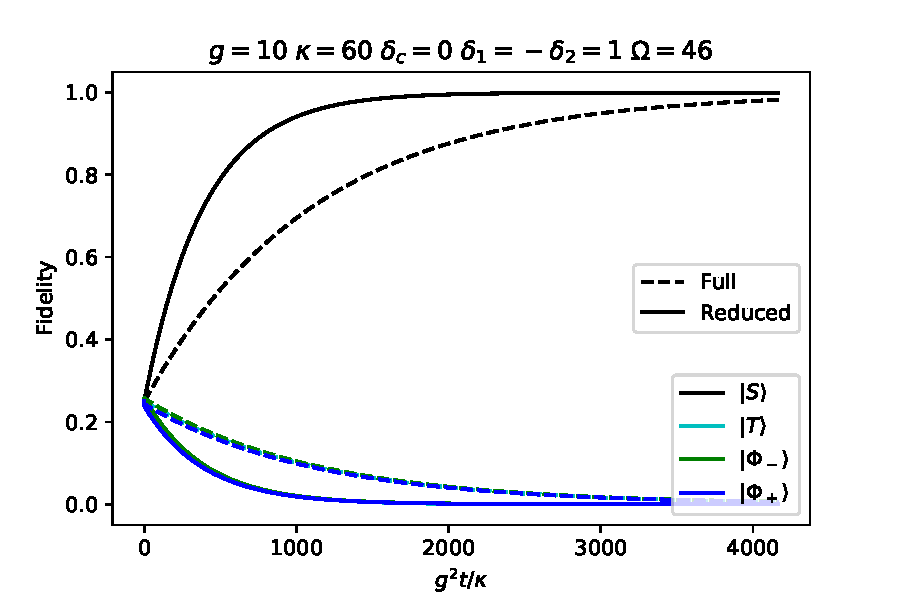
\includegraphics[width=3.5in,height=2.75in]{Sym_stabilization.pdf}
}

\caption{(a) Graphical depiction of two qubits coupled to a lossy resonator mode. (b) After the resonator mode is adiabatically eliminated the resonator decay (red) and the resonator-qubit interactions (blue) merge to create an engineered dissipator (purple). This ``engineered" dissipator gives rise to local qubit relaxation and a dissipative interaction between qubits. (c) Graphical depiction of how the states couple for homogeneous drives and couplings. (d) Master equation simulations of both the full and reduced systems, show high-fidelity stabilization of a singlet state for strong resonant drives.}
\label{LevelDiagram}
\end{figure}
%
\begin{figure} 
\subfigure[]{
\begin{tikzpicture}[x=1.0in,y=1.0in]
\filldraw[color=green!100, fill=green!20 , ultra thick] (0,0) parabola (0.6,1.08) ;
\filldraw[color=green!100, fill=green!20 , ultra thick] (0.0,0.0) parabola (-0.6,1.08) ;
\draw[teal , ultra thick , tipA-tipA] (-.7, -1) -- (.7, -1) ;
\node at (0, -0.8) {\scalebox{1.25}{$J$}} ;
\filldraw[color= magenta!100, fill=magenta!20, ultra thick](-1,-1) circle (.3);
\filldraw[color=magenta!100, fill=magenta!20, ultra thick](1,-1) circle (.3);
\filldraw[color=green!20, fill=green!20] (0,0) -- ( -0.6,1.08) -- ( 0.6,1.08);
\draw[blue, ultra thick , tipA-tipA] (-0.8,-.7) -- (-0.3,0.1);
\draw[blue, ultra thick , tipA-tipA] (0.8,-.7) -- (0.3,0.1);
\node at (.7, -.2) {\scalebox{1.25}{$g$}} ;
\node at (-.7, -.2) {\scalebox{1.25}{$g$}} ;
\node at (-.95,.575) {\scalebox{1.25}{$\kappa$}} ;
\draw [red, ultra thick,-tipA,decorate,decoration={snake,post length=1.65mm}] (-.5,.75) -- (-1.2, .1);
\draw[color= magenta!100 , ultra thick] (-.85,-1.15)--(-1.15,-1.15);
\draw[color= magenta!100 , ultra thick] (-.85,-.85)--(-1.15,-0.85);
\draw[color= magenta!100 , ultra thick] (.85,-1.15)--(1.15,-1.15);
\draw[color= magenta!100 , ultra thick] (.85,-.85)--(1.15,-0.85);
\draw [dashed,color= magenta!100 , ultra thick] (.85,-.90)--(1.15,-0.90);
\draw [dashed,color= magenta!100 , ultra thick] (-.85,-.80)--(-1.15,-0.80);
\draw [gray, ultra thick , tipA-tipA] (-1.0,-1.15)--(-1.0,-.8);
\draw [gray, ultra thick , tipA-tipA] (1.0,-1.15)--(1.0,-.9);
\node at (-0.9,-1.0) {\scalebox{1.0}{$\Omega$}} ;
\node at (0.9,-1.0) {\scalebox{1.0}{$\Omega$}} ;
\node at (-1.37,-0.85) {\scalebox{1.0}{$+\delta$}} ;
\node at (1.37,-0.85) {\scalebox{1.0}{$-\delta$}} ;
\draw[color=green!100 , ultra thick] (-0.36514837167011072,.4) -- (0.36514837167011072,.4);
\draw[color=green!100 , ultra thick] (0.2581988897471611,.2) -- (-0.2581988897471611,.2);
\draw[color=green!100 , ultra thick] (0.44721359549995793,.6) -- (-0.44721359549995793,.6);
\draw[color=green!100 , ultra thick] (0.5163977794943222,.8) -- (-0.5163977794943222,.8);
\draw[color=green!100 , ultra thick] (0.57735026918962573,1.0) -- (-0.57735026918962573,1.0);
\end{tikzpicture}
}
\hspace*{-.3in}
\subfigure[]{
\raisebox{-2cm}{
\begin{tikzpicture}[x=1.0in,y=1.0in]
\filldraw[color= magenta!100, fill=magenta!20, ultra thick](-.6,-1) circle (.3);
\filldraw[color=magenta!100, fill=magenta!20, ultra thick](1.4,-1) circle (.3);
\draw[color= magenta!100 , ultra thick] (-.45,-1.15)--(-0.75,-1.15);
\draw[color= magenta!100 , ultra thick] (-.45,-.85)--(-0.75,-0.85);
\draw[color= magenta!100 , ultra thick] (1.25,-1.15)--(1.55,-1.15);
\draw[color= magenta!100 , ultra thick] (1.25,-.85)--(1.55,-0.85);
\draw[ violet , ultra thick  , -tipA] (-.3, -1.0) --(1.1,-1.0);
%\draw[orange , ultra thick , dashed , tipA-] (-.3, -1.15) --(1.1,-1.15);
\draw[violet , ultra thick , -tipA , decorate , decoration={snake,post length=1.65mm}] (-.6, -1.3) --(-.6,-2.2);
\draw[violet , ultra thick , -tipA , decorate , decoration={snake,post length=1.65mm}] (1.4, -1.3) --(1.4,-2.2);
   \def\mypath{ (-.3, -1.0) --(1.1,-1.0)}
    \draw[color=violet ,  ultra thick , -tipA] \mypath;
    \begin{scope}[overlay]
      \clip (-1, -1) -- \mypath -- ++(1, 0) -- ++(0, -2) -- cycle;
      \draw[color=teal, -tipA , ultra thick] \mypath;
    \end{scope}
\node at (-0.5,-1.0) {\scalebox{1.0}{$\Omega$}} ;
\node at (1.3,-1.0) {\scalebox{1.0}{$\Omega$}} ;
\node at (-0.97,-0.85) {\scalebox{1.0}{$+\delta$}} ;
\node at (1.77,-0.85) {\scalebox{1.0}{$-\delta$}} ;
\draw [gray, ultra thick , tipA-tipA] (-0.6,-1.15)--(-0.6,-.8);
\draw [gray, ultra thick , tipA-tipA] (1.4,-1.15)--(1.4,-.9);
\draw [dashed,color= magenta!100 , ultra thick] (1.25,-.90)--(1.55,-0.90);
\draw [dashed,color= magenta!100 , ultra thick] (-.45,-.80)--(-0.75,-0.80);
%\node at (0.4,-.7) {\scalebox{1.5}{$\frac{8\left| g_1 \right| \left| g_2 \right|}{\kappa}$}} ;
\node at (-0.3,-1.7) {\scalebox{1.5}{$\frac{4 g^2}{\kappa}$}} ;
\node at (1.1,-1.7) {\scalebox{1.5}{$\frac{4 g^2}{\kappa}$}} ;
\end{tikzpicture}
}
}

\subfigure[]{
%\raisebox
\begin{tikzpicture}[x=1.0in,y=1.0in]
\draw[ultra thick] (0.3,0.0) -- (0.90,0.0);
\draw[ultra thick] (1.5,-1.0) -- (2.1,-1.0);
\draw[ultra thick] (1.5,0.0) -- (2.1,0.0);
\draw[ultra thick] (1.5,1.0) -- (2.1,1.0);
\node at (0.15,0.0) {\scalebox{1.25}{$\left| S \right\rangle$}} ;
\node at (2.30,-1.0) {\scalebox{1.25}{$\left| gg \right\rangle$}} ;
\node at (2.30,0.0) {\scalebox{1.25}{$\left| T \right\rangle$}} ;
\node at (2.30,1.0) {\scalebox{1.25}{$\left| ee \right\rangle$}} ;
\node at (1.47,.5) {\scalebox{1.25}{$\sqrt{2} \Omega$}} ;
\node at (1.47,-.5) {\scalebox{1.25}{$\sqrt{2} \Omega$}} ;
\node at (2.1,-.5) {\scalebox{1.25}{$\Gamma$}} ;
\node at (2.1,.5) {\scalebox{1.25}{$\Gamma$}} ;
%\node at (6.0,3.0) {\scalebox{1.0}{$\frac{8g^2}{\kappa}$}} ;
%\node at (6.0,1.0) {\scalebox{1.0}{$\frac{8g^2}{\kappa}$}} ;
    \def\mypath{(.93,0) -- (1.47,0)}
    \draw[color=cyan , ultra thick , tipA-tipA] \mypath;
    \begin{scope}[overlay]
      \clip (-1, -1) -- \mypath -- ++(1, 0) -- ++(0, -2) -- cycle;
      \draw[color=teal, tipA-tipA , ultra thick] \mypath;
    \end{scope}
%\draw[cyan, ultra thick , tipA-tipA] (.93,1) -- (1.47,1);
\node at (1.2, 0.15) {\scalebox{1.25}{$ \delta , \Gamma$}};
\draw[gray, ultra thick , tipA-tipA] (1.7,-1) -- (1.7,0);
\draw[gray, ultra thick , tipA-tipA] (1.7,0) -- (1.7,1);
%\draw[gray, ultra thick , tipA-tipA] (4.6,2) -- (4.6,4);
%%\draw[red, ultra thick, tipA-,decorate, decoration={ snake , post length=2mm }  ] (5.4,0) -- (5.4,2);
%%\draw[red, ultra thick, tipA-,decorate, decoration={snake}] (5.4,2) -- (5.4,4);
%\draw [red, ultra thick,-tipA,decorate,decoration={snake,post length=1.65mm}] (5.4,4) -- (5.4,2);
\draw [violet, ultra thick,-tipA,decorate,decoration={snake,post length=1.65mm}] (1.9,0) -- (1.9,-1);
\draw [violet, ultra thick,-tipA,decorate,decoration={snake,post length=1.65mm}] (1.9,1) -- (1.9,0);
\node at (0.55,1.25) {\scalebox{1.0}{$s=0$}} ;
\node at (1.75,1.25) {\scalebox{1.0}{$s=1$}} ;
\draw[->] (-0.05,-1.2) -- (-.05,1.2) node[left] {$S_z$};
\foreach \y in {-1,0,1} \draw[shift={(-0.05,\y)}] (2pt,0pt) --(-2pt,0pt) node[left] {\footnotesize $\y$};
\end{tikzpicture}
}
\hspace*{-.25in}
\subfigure[]{
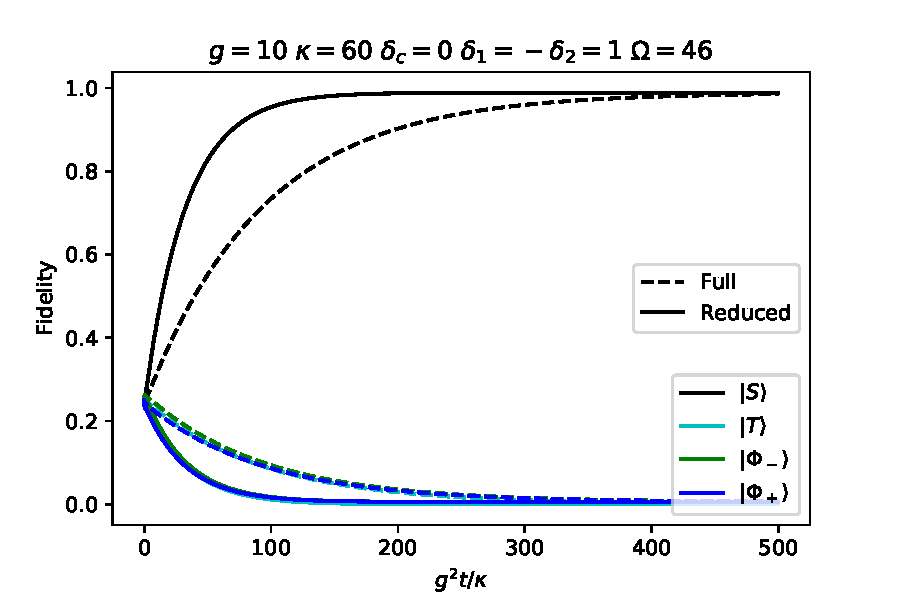
\includegraphics[width=3.5in,height=2.75in]{Asym_stabilization.pdf}
}
\caption{(a) Couplings for implementing chiral interaction between two qubits. The main change from Fig. \ref{LevelDiagram} is addition of the qubit-qubit coupling $J$ (teal arrow). (b) The parametric and dissipative interaction interfere so that the net coupling becomes unidirectional.  (c) The qubit-qubit interaction adds a second coupling between states $|S \rangle \leftrightarrow |T \rangle$ proportional to $\Gamma$. (d) Master equation simulations of both the full and reduced systems, show high-fidelity stabilization of a singlet state for strong resonant drives.}
\label{ChiralLevelDiagram}
\end{figure}
\newpage
%
%ccccccccccccccccccccccccccccccccccccccccccccccccccccccccccc
\subsection{Comparison: Symmetric vs. Chiral}
%cccccccccccccccccccccccccccccccccccccccccccccccccccccccccccc
%
Comparing the stabilization graphs of Fig. \ref{LevelDiagram}(d) and Fig. \ref{ChiralLevelDiagram}(d), we see that the chiral case stabilizes a singlet state significantly faster than its symmetric counterpart by a factor of $\sim8$. The addition of the chiral coupling does cause a decrease in the steady state fidelity, but is more than made up for by the increase in speed. We can capture this idea by defining a performance metric $M$, 
%
\begin{eqnarray}
M = F_{| S \rangle} \frac{\Delta_{\mathcal{L}}}{\Gamma}
\end{eqnarray}
%
that quantifies the product of the fidelity and gap. We first perform an analytical calculation of this quantity for the symmetric case. The fidelity of stabilizing a singlet case can be calculated from the singlet fraction $\alpha = $ introduced earlier as [Eq. (\ref{Two qubit Dark State})], 
%
\begin{eqnarray}
F_{|S\rangle} = \frac{|\alpha|^2}{1+|\alpha|^2} = \frac{\Omega^{2}}{\Omega^{2} + 2\delta^{2}}.
\label{Eq:FidSym}
\end{eqnarray}
%
We can determine the stabilization time by taking the matrix element of Eq. (\ref{Eqn:Formal Dynamical map}) in the singlet state, where $ P_{| S \rangle } = \langle S | \rho | S \rangle$.
%
\begin{equation}
    \dot{P}_{| S \rangle } = \langle S | \mathcal{L} \rho_S | S \rangle.
\end{equation}
%
We adiabatically eliminate the coherences (off-diagonal elements) and solve in terms of the populations so that the rate of preparation of the target state, $|S\rangle$, can be written as \cite{AE_of_coherence, Emery_Paper}
%
\begin{equation}
    \dot{P}_{|S\rangle} = \Gamma_{|g\rangle}P_{|gg\rangle} + \Gamma_{|S\rangle} P_{|S\rangle} + \Gamma_{|T\rangle} P_{|T\rangle} + \Gamma_{|ee \rangle} P_{|ee\rangle}.
\end{equation}
%
Since the ground (or excited) state is farthest from the target state, one can obtain an upper bound for the stabilization rate by considering the rate of preparation of singlet if the system is initialized in $\rho_{S}(0)=|gg\rangle\langle gg|$, i.e. $\Gamma_{|gg\rangle} \geq \Delta_{\mathcal{L}}$ \cite{Emery_Paper}. For the symmetric case,
%
\begin{equation}
    \Delta_{\mathcal{L}} \leq \Gamma_{|gg\rangle} \approx \frac{\Gamma^3}{\Gamma^2 + 2 \Omega^2}.
\label{Eq:GammaSym}
\end{equation}
%
where we have performed a series expansions in the small parameter $\delta/\Omega$ and retained only the zeroth order term. Fig. \ref{fig:Sym_v_Chiral_Timescales}(a) shows a plot of the metric $M$ calculated using Eqs. (\ref{Eq:FidSym}) and (\ref{Eq:GammaSym}) for the symmetric scheme, and compares it with the values obtained from a master equation simulation of the reduced system.
%
\begin{figure}
\subfigure[]{
\centering
%\textbf{       $g=10.0$ $\kappa=60.0$ $\delta=1.0$ $\Omega=10.0$}\par\medskip
\hspace*{-.25in}
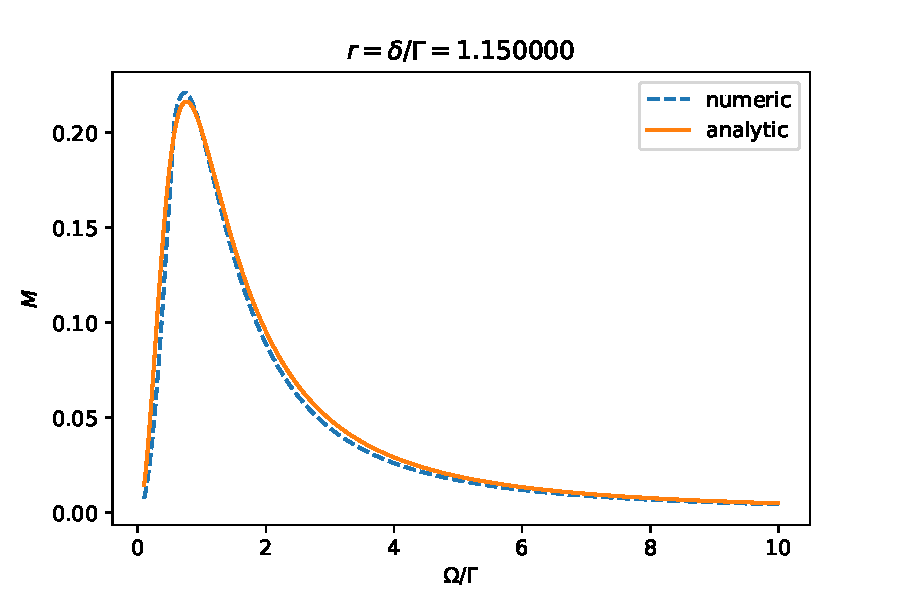
\includegraphics[width=3.0in,height=2.75in]{Images/Sym_Anal_Num.pdf}}
\subfigure[]{
 \centering
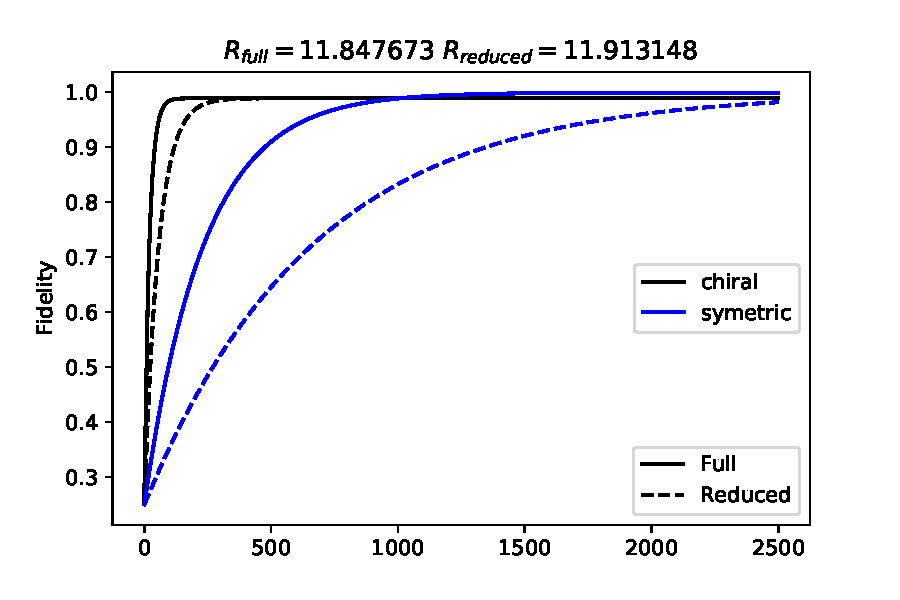
\includegraphics[width=3.0in,height=2.75in]{Images/Sym_v_Chiral.pdf}}
\caption{(a) Performance metric $M=F_{|S\rangle} \Delta_{\mathcal{L}}/\Gamma$ for the symmetric case, plotted as a function of $\Omega/\Gamma$. The agreement between analytical and numerical results is good, though deviations can be seen away from optimal $\Omega/\Gamma$. (b) Performance metric $M$ for chiral scheme is better by a factor of $R=\frac{M_{chiral}}{M_{sym}}\sim 12$, as seen from calculations performed for both the full and reduced system. The parameters used for simulations are the same as that used to generate Figs. \ref{LevelDiagram}(d) and \ref{ChiralLevelDiagram}(d).}
\label{fig:Sym_v_Chiral_Timescales}
\end{figure}
%
\par
%
Fig.~\ref{fig:Sym_v_Chiral_Timescales}(b) shows a comparison of the symmetric and chiral schemes for the same system parameters. As is evident, chiral scheme performs quantitatively better as captured by the ratio of the performance metrics 
%
\begin{eqnarray}
    R = \frac{M_{\rm chiral}}{M_{\rm sym}} \approx 12.
\end{eqnarray}
%